% !TeX encoding = UTF-8
% !TeX spellcheck = en_US
\section{Case studies}

This section presents two case studies to demonstrate the design of linear and nonlinear MPCs. The objective here is to hopefully demonstrate how the package syntax facilitates the implementation and testing of predictive controllers. The first example details how to apply a MPC on a plant at each time step. The second uses higher-level functionalities to quickly simulate closed-loop systems. 

\subsection{Linear Design: Continously Stirred Tank Reactor}

\subsubsection{Linear Model}

The example considers a continuously stirred tank reactor with a cold and hot water intakes, fed at a respective flow rate of $u_c$ and $u_h$. The manipulated input vector is thus $\mathbf{u} = [\begin{smallmatrix}u_c & u_h\end{smallmatrix}]'$. The liquid level $y_L$ and temperature $y_T$ constitute the measured output vector $\mathbf{y} = [\begin{smallmatrix}y_L & y_T\end{smallmatrix}]'$. The figure 1 depicts the instrumentation installed on the plant.

At the steady-state operating point $u_c=u_h=20$, $y_L=50$, and $y_T=30$, the following linear model accurately describes the plant dynamics:
\begin{equation}
\mathbf{G}(s) = \frac{\mathbf{y}(s)}{\mathbf{u}(s)} =
\begin{bmatrix}
    \frac{1.90}{18s+1} & \frac{1.90}{18s+1} \\[3pt]
    \frac{-0.74}{8s+1} & \frac{0.74}{8s+1}
\end{bmatrix}
\end{equation}
The syntax for a sampling time of $T_s=\SI{2}{\second}$ is:
\begin{minted}{julia}
using ModelPredictiveControl, ControlSystemsBase
G = [ tf(1.90, [18, 1]) tf(1.90, [18, 1]);
      tf(-0.74,[8, 1])  tf(0.74, [8, 1]) ]
Ts = 2.0; uop=[20, 20]; yop=[50, 30]
model = setop!(LinModel(G, Ts); uop, yop)
\end{minted}
\spacerepl
\begin{minted}{julia-repl}
Discrete-time linear model with a sample time Ts = 2 s and:
 2 manipulated inputs u
 2 states x
 2 outputs y
 0 measured disturbances d
\end{minted}
The \texttt{model} object will be used for two purposes : to construct our controller, and as a plant simulator to test the design.

\subsubsection{Linear Model Predictive Controller}

The objective is to control both the water temperature and level while constraining the level above 45:

\begin{minted}{julia}
nint_u = [1, 1]; ymin = [45, -Inf]
mpc = setconstraint!(LinMPC(model; nint_u); ymin)
\end{minted}
\spacerepl
\begin{minted}{julia-repl}
LinMPC controller with a sample time Ts = 2.0 s,
OSQP optimizer, SteadyKalmanFilter estimator and:
 10 prediction steps Hp
  2 control steps Hc
  2 manipulated inputs u (2 integrating states)
  4 states x̂
  2 measured outputs ym (0 integrating states)
  0 unmeasured outputs yu
  0 measured disturbances d
\end{minted}

By default, \texttt{LinMPC} controllers use \texttt{OSQP.jl} to solve the problem, soft constraints on output predictions $\mathbf{\hat y}$ to ensure feasibility, and a \texttt{SteadyKalmanFilter} to estimate the plant states\footnote{As an alternative to state observer, we could have use an internal model structure with \texttt{estim = InternalModel(model)} and \texttt{mpc = setconstraint!(estim; nint\_u); ymin)}. It was tested on this example and it gives similar results.}. An attentive reader will also notice that the Kalman filter estimates two additional states compared to the plant model. These are the integrating states for the unmeasured plant disturbances, added at the inputs $\mathbf{u}$ for this example.

Before closing the loop, the actual plant inputs and measurements should initialize the estimates to ensure a bumpless transfer. Since the plant is the linear model here, its output will initialize the states. \texttt{LinModel} objects are callable for this purpose. Once done, imposing step changes on the setpoint $\mathbf{r_y}$ and on a load disturbance $u_l$ tests the closed-loop performance of \texttt{mpc}:
\begin{minted}{julia}
function test_mpc(mpc, plant)
    plant.x[:] .= 0; y = plant() # or evaloutput(plant)
    initstate!(mpc, plant.uop, y)
    N = 75; ry = [50, 30]; ul = 0
    U, Y, Ry = zeros(2, N), zeros(2, N), zeros(2, N)
    for i = 1:N
        i == 26 && (ry = [48, 35])
        i == 51 && (ul = -10)
        y = plant() # simulations
        u = mpc(ry) # or moveinput!(mpc, ry)
        U[:,i], Y[:,i], Ry[:,i] = u, y, ry
        updatestate!(mpc, u, y) # update mpc estimate
        updatestate!(plant, u+[0,ul]) # update simulator
    end
    return U, Y, Ry
end
U_data, Y_data, Ry_data = test_mpc(mpc, model)
\end{minted}
Updating the internal states of \texttt{mpc} prepares the object for the \emph{next} time step. That is why the call is done at the end of the \texttt{for} loop. The same logic applies for \texttt{model}. Lastly, we plot the closed-loop test with \texttt{Plots.jl}:
\begin{minted}{julia}
res = SimResult(mpc, U_data, Y_data; Ry_data)
using Plots; plot(res)
\end{minted}
\cref{fig:plot1_LinMPC} shows that the controller violates the constraints around 110 s because of the disturbance. Adding feedforward compensation can mitigate this.

\begin{figure}
    \centering
    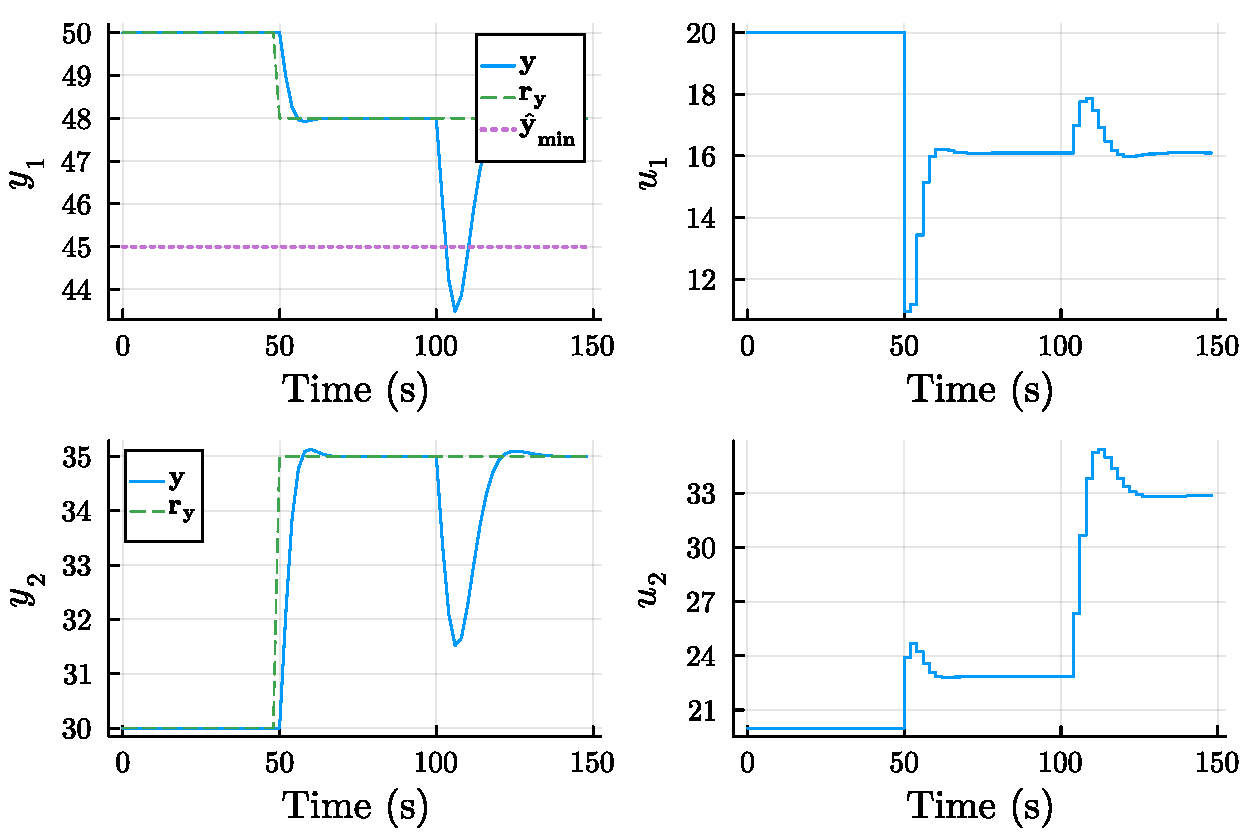
\includegraphics[width=\columnwidth]{fig/plot1_LinMPC.pdf}
    \caption{CSTR closed-loop simulation}
    \label{fig:plot1_LinMPC}
\end{figure}

\subsubsection{Feedforward Compensation}

Suppose that the load disturbance $u_l$ of the last section is in fact caused by a separate hot water pipe that discharges into the tank. Measuring this flow rate allows us to incorporate feedforward compensation (FF):

\begin{minted}{julia}
model_ff = LinModel([G G[1:2, 2]], Ts; i_d=[3])
model_ff = setop!(model_ff; uop, yop, dop=[20])
\end{minted}
\spacerepl
\begin{minted}{julia-repl}
Discrete-time linear model with a sample time Ts = 2 s and:
 2 manipulated inputs u
 4 states x
 2 outputs y
 1 measured disturbances d
\end{minted}
The simulation needs a new \texttt{LinMPC} object based on \texttt{model\_ff} and a new test function that employs the current disturbance measurement:
\begin{minted}{julia}
mpc_ff = setconstraint!(LinMPC(model_ff; nint_u); ymin)
function test_mpc_ff(mpc_ff, plant)
    plant.x[:] .= 0; y = plant(); d = [20]
    initstate!(mpc_ff, plant.uop, y, d)
    N = 75; ry = [50, 30]; ul = 0
    U, Y, Ry = zeros(2, N), zeros(2, N), zeros(2, N)
    Ry_data = zeros(2, N)
    for i = 1:N
        i == 26 && (ry = [48, 35])
        i == 51 && (ul = -10)
        y, d = plant(), [20+ul] # simulations
        u = mpc_ff(ry, d) # d in arguments
        U[:,i], Y[:,i], Ry[:,i] = u, y, ry
        updatestate!(mpc_ff, u, y, d) # d in arguments
        updatestate!(plant, u+[0,ul])
    end
    return U, Y, Ry
end
U_data, Y_data, Ry_data = test_mpc_ff(mpc_ff, model)
res = SimResult(mpc, U_data, Y_data; Ry_data)
plot(res)
\end{minted}

\cref{fig:plot2_LinMPC} shows that the feedforward compensation handles the disturbance without violating the constraint.

\begin{figure}
    \centering
    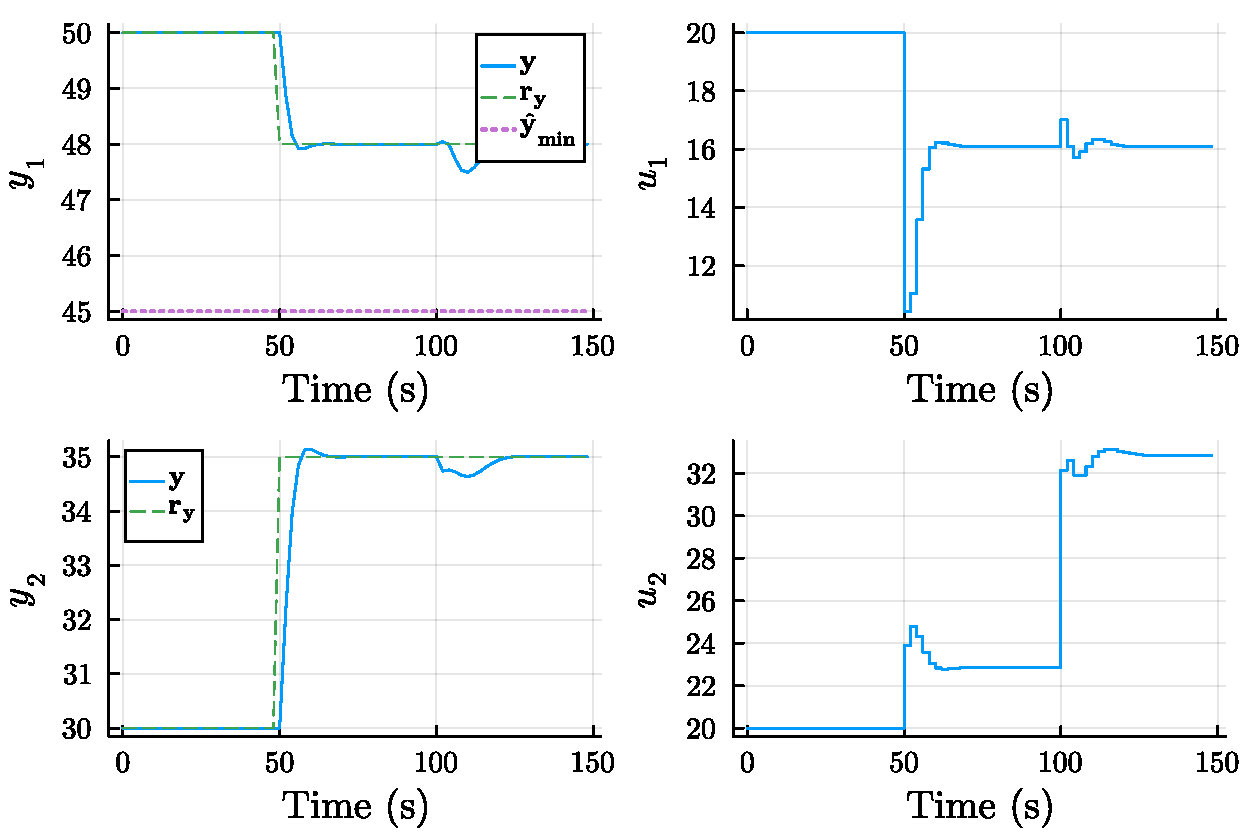
\includegraphics[width=\columnwidth]{fig/plot2_LinMPC.pdf}
    \caption{CSTR closed-loop simulation with feedforward}
    \label{fig:plot2_LinMPC}
\end{figure}

\subsection{Nonlinear Design : Inverted Pendulum}

In this ex

\section{Results and Discussion}
\label{sec.results_simple}

Laboris exercitation sunt adipisicing laboris nulla ad occaecat irure magna voluptate. Veniam eu labore Lorem anim nostrud minim Lorem fugiat nulla. Non anim veniam laborum deserunt adipisicing cillum aliquip deserunt pariatur consectetur consequat irure. Dolor aute incididunt quis magna. Dolor nostrud exercitation duis sunt nulla adipisicing enim laborum ex ut esse ad. Incididunt exercitation velit ea elit ut laboris eu amet.

Minim magna culpa ipsum do proident cillum sit. Officia ad et consequat do magna nostrud irure nostrud. Ipsum sunt adipisicing Lorem sunt tempor ex veniam consequat veniam ipsum. Aliquip voluptate labore mollit duis id mollit nulla id ipsum. Velit esse nisi qui pariatur ad nostrud.

Aute minim anim culpa minim aliquip sint laboris sunt. Ea ex tempor irure officia laborum est aliquip nostrud quis do. Lorem cupidatat mollit do officia aute in est cillum cillum consectetur laborum pariatur. Id tempor minim eiusmod ex laboris. Aute aliquip cupidatat nostrud aute dolor mollit ex commodo do excepteur dolor irure. Ut veniam amet id excepteur excepteur velit laboris aliqua sit occaecat irure dolor labore.

Proident ad minim magna minim excepteur reprehenderit elit id ipsum amet velit sunt aute aute. Consectetur excepteur velit quis aliqua sint laborum veniam minim proident. Veniam proident laboris aute deserunt do do amet qui pariatur occaecat cillum. Minim magna in et laborum ipsum deserunt pariatur cupidatat ipsum veniam aliqua elit. Aliqua id proident fugiat nisi esse eu nulla sint qui reprehenderit aliqua sunt. Cillum duis anim sit velit dolore.

\begin{table}[tb]
	\caption{Simplified model parameters for batch fluidized bed drying}
	\label{tab.simple_params}
	\centering
	% !TeX spellcheck = en_US

\begin{tabular}{l l l l}
	
\toprule %=======================================================================

parameter 			& value 	   		& \shortstack[l]{standard\\deviation} & units  \\

\midrule %-----------------------------------------------------------------
					
\glsub{chi}{0}    	& \num{0.15e-2}		& -- 					& --		\\

%--------------------------------------------------------------------------

\rowcolor{blue!10}
\gls{a1}			& \num{9.26e-5}		& \num{0.04e-5}		%
										& \si{\per\meter\cubed} \\
\rowcolor{blue!10}
\gls{b1}			& \num{4.54e-2}		& \num{0.05e-2}		%
										& \si{\degreeCelsius\per\meter\cubed} \\
\rowcolor{blue!10}					
\gls{b2}			& \num{2.56e-05}	& \num{0.02e-05}	%
										& \si{\per\meter\cubed}	 \\

%--------------------------------------------------------------------------

\rowcolor{blue!10}
\gls{nu}			& \num{3.48}		&  \num{0.12}		& -- \\		
\rowcolor{blue!10}
\glsub{chi}{pc}		& \num{2.33e-2}	 	&  \num{0.06e-2}	& -- \\
				
%-------------------------------------------------------------------------

\gls{alpha}   	   	& \num{4.90e-3} 	& --			& --  \\
\gls{beta}			& \num{5.70e-2}		& -- 			& \si{\per\degreeCelsius}\\

%----------------------------------------------------------------------------

\gls{tau}			& \num{86.7}		&--				& \si{\second}  \\

\bottomrule %====================================================================
	
\end{tabular}

\end{table}

Occaecat Lorem commodo in minim consectetur voluptate nostrud enim tempor incididunt laborum occaecat. Aliqua non et nulla voluptate amet sunt. Laboris nisi consequat cupidatat est consequat deserunt ipsum.
